\documentclass[a4paper]{article}
\usepackage{tikz}
\usepackage{mathtools}
\usepackage{caption}
\usetikzlibrary{graphs}
\DeclarePairedDelimiter{\ceil}{\lceil}{\rceil}
\usepackage{listings}
\usepackage{color}
\usepackage{soul}

\definecolor{dkgreen}{rgb}{0,0.6,0}
\definecolor{gray}{rgb}{0.5,0.5,0.5}
\definecolor{mauve}{rgb}{0.58,0,0.82}
\definecolor{darkblue}{rgb}{0.0,0.0,0.6}
\definecolor{cyan}{rgb}{0.0,0.6,0.6}

 \lstset{frame=tb,
  language=Java,
  breaklines=true,
  showstringspaces=false,
  columns=flexible,
  numbers=none,
  commentstyle=\color{dkgreen},
  stringstyle=\color{mauve},
  tabsize=3
}
\begin{document}
	\title{Design and Implementation of Steiner Tree for Network Graph}
	\author{Harshavardhan Nalajala}
	\date{}
	\maketitle
	\tableofcontents

\section{Steiner Minimum Tree}
Given an undirected graph G(V, E, W) and S $\subseteq$ V, where V is the set of vertices, E is the set of edges and W is the set of non negative weights associated with the edges of the graph , tree(T) spanning S such that $\sum_{e \in T}$ l(e) is minimum, is known as a steiner tree for the graph \cite{BOOK}. The subset {S} is called terminal set while any subset of {V} used to generate {T} is called steiner subset. Steiner trees are important in various applications such as VLSI routing, wirelength estimation, and network routing.
Two variants of Steiner Tree can further be defined.
\begin{itemize}
\item Minimum Spanning Tree: If {S} is equal to {V}, the steiner tree thus obtained in minimum spanning tree which spans all of the vertices of the graph {G}.
\item Shortest Path: If cardinality of the subset {S} is exactly equal to 2, then steiner tree thus obtained is the shortest path between the two vertices in the subset {S}.
\end{itemize}
However while both variants are solvable in polynomial time, the decision variant of steiner tree problems is {NP-complete} and hence optimization problem is {NP-hard}. This was shown by a transformation from the EXACT COVER BY 3-SETS problem \cite{NP}. Many versions of Steiner Tree exist such as 
\begin{itemize}
\item Euclidean Steiner Tree where {'N'} points are given and the goal is the connect them using lines of minimum length either directly or via other points and line segments. For N = 3 there are two possible cases: if the triangle formed by the given points has all angles which are less than 120 degrees, the solution is given by a Steiner point located at the Fermat point; otherwise the solution is given by the two sides of the triangle which meet on the angle with 120 or more degrees. For general N, the Euclidean Steiner tree problem is NP-hard.
\item Rectilinear Steiner Tree where euclidean distances are replaced by rectilinear distances. The problem arises in the physical design of electronic design automation.
\end{itemize}
\begin{figure}
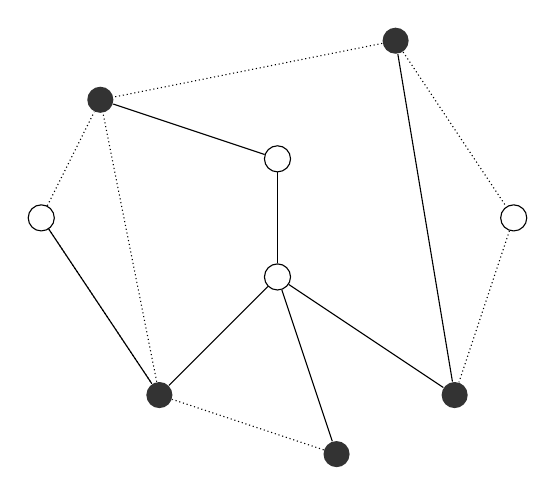
\begin{tikzpicture}
  [scale=.75,auto=left,every node/.style={circle,fill=black!20}]
  \node[fill=white, draw, rounded corners] (n8) at (-4,1) {};
  \node[fill=black!80] (n6) at (-2, -2) {};
  \node[fill=black!80] (n7) at (1,-3) {};
  \node[fill=white, draw, rounded corners] (n4) at (0,0)  {};
  \node[fill=white, draw, rounded corners] (n5) at (0,2)  {};
  \node[fill=black!80] (n1) at (2,4) {};
  \node[fill=white, draw, rounded corners] (n2) at (4,1)  {};
  \node[fill=black!80] (n3) at (3,-2)  {};
  \node[fill=black!80] (n0) at (-3, 3) {};

  \foreach \from/\to in {n6/n4, n8/n6, n7/n4, n4/n5, n5/n0, n3/n4, n3/n1}
    \draw (\from) -- (\to);
   \foreach \from/\to in {n8/n6, n8/n0, n6/n0, n7/n6, n1/n0, n2/n3, n1/n2}
    \draw[densely dotted] (\from) -- (\to);
\end{tikzpicture}
\caption{A graph minimal steiner tree. Black points are terminals and white points are steiner points}
\label{graph1}
\end{figure}

\section{Approximation by MST}
Since the decision variant of SMT(Steiner Minimum Tree) problem is NP-complete, we need to focus on approximation results. A well-known method to approximate an SMT is to use a minimal spanning tree (MST). First we construct the metric closure on S, i.e., a complete graph with vertices S and edge weights equal to the shortest path lengths. Then we find an MST on the closure, in which each edge corresponds to one shortest path on the original graph. Finally the MST is transformed back to a Steiner tree by replacing each edge with the shortest path and some straightforward postprocessing to remove any possible cycle \cite{MST}.

\subsection{Algorithm}
Input: A graph G = (V, E, W) and a terminal set S$\subseteq$ V \\
Output: T\textsubscript{SMT}
\begin{itemize}
\item Construct the metric closure, G\textsuperscript{'} on the terminal set S.
\item Use PRIM's minimum spanning tree algorithm on G\textsuperscript{'} and find the minimum spanning tree T\textsuperscript{'}\textsubscript{MST}.
\item for each edge e in E(T\textsuperscript{'}\textsubscript{MST}) in a depth-first-search order: 
\begin{itemize}
\item Find a shortest path SP from u to v on G.
\item if vertices in SP have not already been added to T\textsubscript{SMT}, add vertices to T\textsubscript{SMT}.
\item if cycles are formed, Use PRIM's minimum spanning tree algorithm and remove cycles.
\end{itemize}
\end{itemize}

\begin{figure}
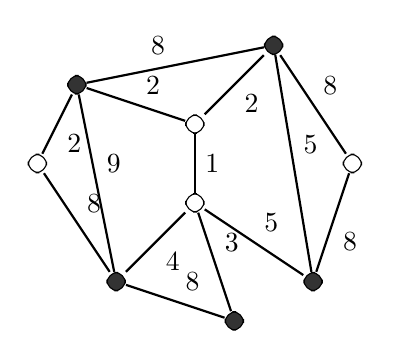
\begin{tikzpicture}
  [scale=.5,auto=left]
      \tikzstyle{edge_style} = [draw=black, line width=2, thick]
  \node[fill=white, draw, rounded corners] (n8) at (-4,1) {};
  \node[fill=black!80, draw, rounded corners] (n6) at (-2, -2) {};
  \node[fill=black!80, draw, rounded corners] (n7) at (1,-3) {};
  \node[fill=white, draw, rounded corners] (n4) at (0,0)  {};
  \node[fill=white, draw, rounded corners] (n5) at (0,2)  {};
  \node[fill=black!80, draw, rounded corners] (n1) at (2,4) {};
  \node[fill=white, draw, rounded corners] (n2) at (4,1)  {};
  \node[fill=black!80, draw, rounded corners] (n3) at (3,-2)  {};
  \node[fill=black!80, draw, rounded corners] (n0) at (-3, 3) {};
  \draw[edge_style] (n0) edge node {8} (n1);
    \draw[edge_style] (n0) edge node {2} (n5);
  \draw[edge_style] (n0) edge node {2} (n8);
  \draw[edge_style] (n0) edge node {9} (n6);
  \draw[edge_style] (n1) edge node {2} (n5);
  \draw[edge_style] (n1) edge node {8} (n2);
  \draw[edge_style] (n1) edge node {5} (n3);
  \draw[edge_style] (n5) edge node {1} (n4);
  \draw[edge_style] (n4) edge node {4} (n6);
  \draw[edge_style] (n4) edge node {3} (n7);
  \draw[edge_style] (n4) edge node {5} (n3);
  \draw[edge_style] (n6) edge node {8} (n7);
  \draw[edge_style] (n8) edge node {8} (n6);
  \draw[edge_style] (n2) edge node {8} (n3);
\end{tikzpicture}
\caption{Example Graph}
\label{example}
\end{figure}
\subsection{Example}
Consider the graph(G) depicted in figure \ref{example}. V consists of 9 vertices, E consists of 14 edges, and subset S consists of 5 vertices. Goal is to find the steiner tree that spans over S. Metric closure of G, given by G\textsuperscript{'} is calculated by using shortest path algorithm and is depicted in figure \ref{metric}.
\begin{figure}
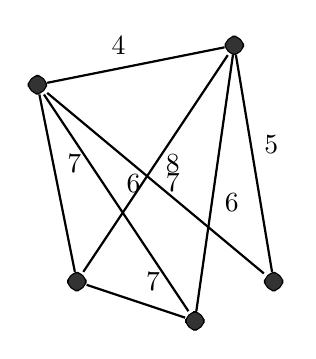
\begin{tikzpicture}
  [scale=.5,auto=left]
      \tikzstyle{edge_style} = [draw=black, line width=2, thick]
  \node[fill=black!80, draw, rounded corners] (n6) at (-2, -2) {};
  \node[fill=black!80, draw, rounded corners] (n7) at (1,-3) {};
  \node[fill=black!80, draw, rounded corners] (n1) at (2, 4) {};
  \node[fill=black!80, draw, rounded corners] (n3) at (3,-2)  {};
  \node[fill=black!80, draw, rounded corners] (n0) at (-3, 3) {};
  \draw[edge_style] (n0) edge node {4} (n1);
    \draw[edge_style] (n0) edge node {8} (n3);
  \draw[edge_style] (n0) edge node {6} (n7);
  \draw[edge_style] (n0) edge node {7} (n6);
  \draw[edge_style] (n1) edge node {7} (n6);
  \draw[edge_style] (n1) edge node {6} (n7);
  \draw[edge_style] (n1) edge node {5} (n3);
  \draw[edge_style] (n6) edge node {7} (n7);
\end{tikzpicture}
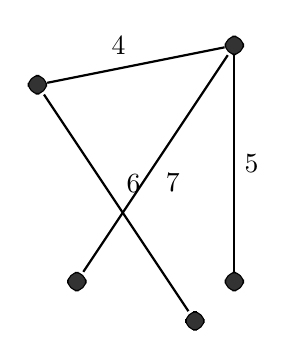
\begin{tikzpicture}
  [scale=.5,auto=left]
      \tikzstyle{edge_style} = [draw=black, line width=2, thick]
  \node[fill=black!80, draw, rounded corners] (n6) at (22, -2) {};
  \node[fill=black!80, draw, rounded corners] (n7) at (25,-3) {};
  \node[fill=black!80, draw, rounded corners] (n1) at (26,4) {};
  \node[fill=black!80, draw, rounded corners] (n3) at (26,-2)  {};
  \node[fill=black!80, draw, rounded corners] (n0) at (21, 3) {};
  \draw[edge_style] (n0) edge node {4} (n1);
  \draw[edge_style] (n0) edge node {6} (n7);
  \draw[edge_style] (n1) edge node {7} (n6);
  \draw[edge_style] (n1) edge node {5} (n3);
\end{tikzpicture}

\caption{Metric Closure of Graph in Figure \ref{example} and its T\textsuperscript{'}\textsubscript{MST}}
\label{metric}
\end{figure}
Minimum spanning tree(T\textsuperscript{'}\textsubscript{MST}) is obtained by applying PRIM's algorithm over G\textsuperscript{'} as depicted in figure \ref{metric}.
\begin{figure}
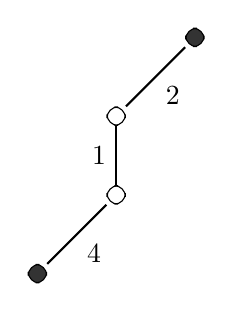
\begin{tikzpicture}
  [scale=.5,auto=left]
      \tikzstyle{edge_style} = [draw=black, line width=2, thick]
  \node[fill=black!80, draw, rounded corners] (n6) at (22, -2) {};
  \node[fill=black!80, draw, rounded corners] (n1) at (26,4) {};
  \node[fill=white, draw, rounded corners] (n4) at (24,0)  {};
  \node[fill=white, draw, rounded corners] (n5) at (24,2)  {};
  \draw[edge_style] (n1) edge node {2} (n5);
  \draw[edge_style] (n4) edge node {1} (n5);
  \draw[edge_style] (n4) edge node {4} (n6);
\end{tikzpicture}
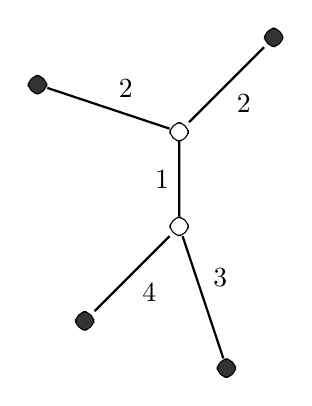
\begin{tikzpicture}
  [scale=.6,auto=left]
      \tikzstyle{edge_style} = [draw=black, line width=2, thick]
  \node[fill=black!80, draw, rounded corners] (n6) at (42, -2) {};
  \node[fill=black!80, draw, rounded corners] (n7) at (45,-3) {};
  \node[fill=black!80, draw, rounded corners] (n1) at (46,4) {};
  \node[fill=white, draw, rounded corners] (n4) at (44,0)  {};
  \node[fill=white, draw, rounded corners] (n5) at (44,2)  {};
  \node[fill=black!80, draw, rounded corners] (n0) at (41, 3) {};
  \draw[edge_style] (n1) edge node {2} (n5);
  \draw[edge_style] (n4) edge node {1} (n5);
  \draw[edge_style] (n4) edge node {4} (n6);
  \draw[edge_style] (n0) edge node {2} (n5);
  \draw[edge_style] (n4) edge node {3} (n7);
\end{tikzpicture}
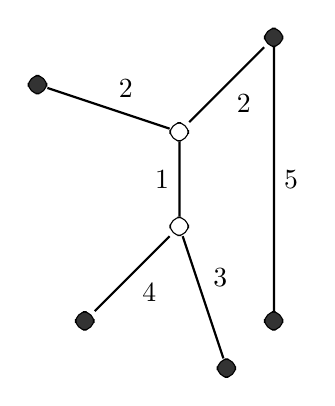
\begin{tikzpicture}
  [scale=.6,auto=left]
      \tikzstyle{edge_style} = [draw=black, line width=2, thick]
  \node[fill=black!80, draw, rounded corners] (n6) at (62, -2) {};
  \node[fill=black!80, draw, rounded corners] (n7) at (65,-3) {};
  \node[fill=black!80, draw, rounded corners] (n1) at (66,4) {};
  \node[fill=white, draw, rounded corners] (n4) at (64,0)  {};
  \node[fill=white, draw, rounded corners] (n5) at (64,2)  {};
  \node[fill=black!80, draw, rounded corners] (n0) at (61, 3) {};
  \node[fill=black!80, draw, rounded corners] (n3) at (66,-2)  {};

  \draw[edge_style] (n1) edge node {2} (n5);
  \draw[edge_style] (n4) edge node {1} (n5);
  \draw[edge_style] (n4) edge node {4} (n6);
  \draw[edge_style] (n0) edge node {2} (n5);
  \draw[edge_style] (n4) edge node {3} (n7);
  \draw[edge_style] (n1) edge node {5} (n3);
\end{tikzpicture}
\caption{Expansion of edges in $T^{'}_{MST}$}
\label{path}
\end{figure}
Each edge in $T^{'}_{MST}$ is then expanded in depth first search order and any node not in the tree is added to the tree. Once all paths are enumerated, the tree thus formed, if it has cycles, will further be pruned using PRIM's MST algorithm again. The end result obtained is the steiner tree spanning over subset S and can contain steiner nodes. Figure \ref{path} depicts the edge expansion and tree formation.

\subsection{Complexity}
The running time complexity of the algorithm is O($\vert$V$\vert$$\vert$$S^2$$\vert$). \\
Steiner Ratio is another metric used as a measure of performance of an MST as a polynomial time approximation of the SMT. Steiner ratio is defined as
\begin{equation}
							\rho = \frac{mst(G^{'})}{smt(G, S)}
\end{equation}
Using the metric closure approximation algorithm results in $\rho$ = 2.
\section{Steiner Tree for Network Graph}
A network of nodes can be identified by an undirected graph(G) with set of nodes being vertices(V) and cost of using the path between nodes as weight of the edges between the nodes(E, W).  \par
Steiner tree often arises in network design and wiring layout problems.     Suppose we are given a set of sites that must be connected by wires as cheaply as possible. The minimum Steiner tree describes the way to connect them using the smallest amount of wire. In certain applications, such as minimum cost communications networks, construction costs are high enough to invest large amounts of computation in finding the best possible Steiner tree.\par
The heuristic used gets the cost of using the paths between two nodes using RIP or other shortest path protocols. These costs(E,W) will be used to get the metric closure(G\textsuperscript{'}), $T^{'}_{MST}$ and finally output the steiner tree($T_{SMT}$). Each node has to complete view of the graph using shortest path routing protocols. This view is then used to determine the steiner tree with given set of terminals.\par
\subsection{Data Structures at each node}
Each node maintains a list of {$<$Destination, nextHop$>$}tuple. {Destination} is a terminal while {nextHop} can be either a terminal or a steiner node. Number of terminals determine the complexity of the list with worst case being the set of nodes determined by shortest path based protocols.

\section{Implementation of Steiner Tree}
INPUT: Network Graph, G(V, E, W) along with subset of terminals, S. Input file contains the following.\\
First line V E S \\
E lines of edge weights in the format v\textsubscript{i} v\textsubscript{j} w\textsubscript{ij}\\
Next line contains S terminals s\textsubscript{i}\\

\subsection{Definitions and declarations}
Data structures and header file.
\begin{lstlisting}
#ifndef __STEINER_TREE_H
#define __STEINER_TREE_H

/* Edge between orig and end with weight value */
typedef struct {
        int orig;
        int end;
        int value;
} edge;

/* Heap to hold edges to return Min/Max weighted edge in O(logE) complexity */
typedef struct {
        int size;
        edge *e;
} heap;

/* Function: debugHeap
 * Arguments: Pointer to the heap Structure
 *      Used to debug data in the heap
 */
void debugHeap(heap *);

/* Function: minHeapify
 * Arguments: Pointer to the heap Structure
 *      Useed to heapify the data such that minimum element is at the root of the heap structure.
 */
void minHeapify(heap *);

/* Function: addToHeap
 * Arguments: Pointer to the heap Structure,
 *              int originatingVertex,
 *              int endVertex,
 *              int weightOfEdge
 */
void addToHeap(heap *, int , int , int );

/* Function: getMinFromHeap
 * Arguments: Pointer to the heap Structure
 *      Used to get minimum element from the heap
 * Return Value: Pointer to the Edge structure
 */
edge *getMinFromHeap(heap *);

/* List of nodes in the path between two vertices */
typedef struct node {
        int v;
        struct node *next;
} path;

/* Function: findPath
 * Arguments: int numberOfVertices,
  *              int edgeWeights[totalVertices][totalVertices],
 *              int weightValue,
 *              int startVertex,
 *              int endVertex
 * Return Value: Pointer to the path of startVertex to endVertex with weightValue
 */
path *findPath(int vertices, int localWeights[][vertices], int weight, int startv, int endv);

/* Function: findLGraph
 * Arguments: int numberOfVertices,
 *              int numberOfEdges,
 *              int edgeweights[numberOfVertices][numberOfVertices],
 *              int numberOfTerminals,
 *              int *listOfTerminals,
 *              <OUT> int pathLength[numberOfTerminals][numberOfTerminals]
 *      Function used to find the metric closure of an input graph with edgeweights and outputs
 *      shortest path lengths between vertices in listofterminals.
 */
void findLGraph(int vertices, int edges, int weights[][vertices],
                int *terminalVertices, int terminals, int pathLength[][terminals]);

/* Function: getMinSpanTree
 * Arguments: int numberOfTerminals,
 *              int listOfTerminals[numberOfTerminals],
 *              int edgeweights[numberOfTerminals][numberOfTerminals],
 *              <OUT>int tree[numberOfTerminals][numberOfTerminals]
 *      Function to find the minimum spanning tree of a given graph with weights and outputs the tree.
 *      Algorithm followed: PRIM'S MINIMUM SPANNING TREE
 */
void getMinSpanTree(int terminals, int *terminalVertices, int weights[][terminals], int tree[][terminals]);

/* Function: findSteinerTree
 * Arguments: int numberOfTerminals,
 *              int listOfTerminals[numberOfTerminals],
 *              int minSpanTree[numberOfTerminals][numberOfTerminals],
 *              int numberOfVertices,
 *              int edgeweights[numberOfVertices][numberOfVertices],
 *              <OUT> int minSteinerTree[numberOfVertices][numberOfVertices]
 *      Function used to get the minimum steiner tree from given minimum spanning tree of metric closure obtained
 *      from graph with edgeweights.
 *      Outputs the edgeweights of terminals and steiner points used in the minimum steiner tree.
 */
void findSteinerTree(int terminals, int *terminalVertices, int minSpanTree[][terminals],
                        int vertices, int localWeights[][vertices], int minSteinerTree[][vertices]);
#endif
\end{lstlisting}
\subsection{Implementation of the functions}
\begin{lstlisting}
#include <stdio.h>
#include <limits.h>
#include <stdlib.h>
#include "steinertree.h"

/* Function: debugHeap
 * Arguments: Pointer to the heap Structure
 *      Used to debug data in the heap
 */
void debugHeap(heap *minHeap) {
        int i = 1;
        printf("Heap:");
        while (i <= minHeap->size) {
                printf("%d %d->%d, ", minHeap->e[i].value, minHeap->e[i].orig, minHeap->e[i].end);
                i+=1;
        }
        printf("\n");
}

/* Function: minHeapify
 * Arguments: Pointer to the heap Structure
 *      Useed to heapify the data such that minimum element is at the root of the heap structure.
 */
void minHeapify(heap *minheap) {
        int size = minheap->size;
        edge value = minheap->e[size];
        int parent = size/2;
        int child = size;
        int done = 0;
        while (parent != 0 && !done) {
                /* edge structre contains value, originating vertex, and end vertex.
                 * if parent value is greater than child value, min heap property is violated
                 * so fix by swapping child and parent.
                 * Continue until no such violation is found or we reach root */
                if (minheap->e[parent].value > value.value) {
                        edge temp = minheap->e[parent];
                        minheap->e[parent].value = value.value;
                        minheap->e[parent].orig = value.orig;
                        minheap->e[parent].end = value.end;
                        minheap->e[child].value = temp.value;
                        minheap->e[child].orig = temp.orig;
                        minheap->e[child].end = temp.end;
                        child = parent;
                        parent = parent/2;
                } else {
                        // no element violates min heap property
                        done = 1;
                }
        }
}

/* Function: addToHeap
 * Arguments: Pointer to the heap Structure,
 *              int originatingVertex,
 *              int endVertex,
 *              int weightOfEdge
 */
void addToHeap(heap *minheap, int value, int orig, int end) {
        int size = minheap->size;
        // Add the element to the end of the list and heapify to make sure
        // elements satisfy min heap property
        minheap->e[size+1].value = value;
        minheap->e[size+1].orig = orig;
        minheap->e[size+1].end = end;
        minheap->size = size + 1;
        minHeapify(minheap);
}

/* Function: getMinFromHeap
 * Arguments: Pointer to the heap Structure
 *      Used to get minimum element from the heap
 * Return Value: Pointer to the Edge structure
 */
edge *getMinFromHeap(heap *minheap) {
        int size = minheap->size;
        if (size == 0) {
                return NULL;
        }
        // Element at the first index is the minimum element in the min heap
        edge *value = (edge *)malloc(sizeof(edge));
        value->value = minheap->e[1].value;
        value->orig = minheap->e[1].orig;
        value->end = minheap->e[1].end;
        // copy the last element in the heap
        minheap->e[1].value = minheap->e[size].value;
        minheap->e[1].orig = minheap->e[size].orig;
        minheap->e[1].end = minheap->e[size].end;
        minheap->size = size - 1;
        size--;

        int i = 1;
        while (i < size) {
                // Make sure min heap property is satisfied on removing the root of the heap.
                if (2*i > size || 2*i+1 > size) {
                        break;
                }
                int v = minheap->e[i].value;
                int orig = minheap->e[i].orig;
                int end = minheap->e[i].end;
                int lchild = minheap->e[2*i].value;
                int lchild = minheap->e[2*i].value;
                int rchild = minheap->e[2*i +1].value;

                // check root with left child and right child.
                // if root value is greater than left child, left child is less than right child,
                // swap root and left child. Goto left and redo until end of heap or no violator is found.
                if (v > lchild && lchild <= rchild) {
                        minheap->e[i].value = minheap->e[2*i].value;
                        minheap->e[i].orig = minheap->e[2*i].orig;
                        minheap->e[i].end = minheap->e[2*i].end;
                        minheap->e[2*i].value = v;
                        minheap->e[2*i].orig = orig;
                        minheap->e[2*i].end = end;
                        i = 2*i;
                } else if (v > rchild && rchild <= lchild) {
                        // if root value is greater than right child, right child is less than left child,
                        // swap root and right child. Goto right and redo until end of heap or no violator is found.
                        minheap->e[i].value = minheap->e[2*i+1].value;
                        minheap->e[i].orig = minheap->e[2*i+1].orig;
                        minheap->e[i].end = minheap->e[2*i+1].end;
                        minheap->e[2*i+1].value = v;
                        minheap->e[2*i+1].orig = orig;
                        minheap->e[2*i+1].end = end;
                        i = 2*i + 1;
                } else {
                        // no violator of min heap property is found
                        break;
                }
        }
        return value;
}

/* Function: findLGraph
 * Arguments: int numberOfVertices,
 *              int numberOfEdges,
 *              int edgeweights[numberOfVertices][numberOfVertices],
 *              int numberOfTerminals,
 *              int *listOfTerminals,
 *              <OUT> int pathLength[numberOfTerminals][numberOfTerminals]
 *      Function used to find the metric closure of an input graph with edgeweights and outputs
 *      shortest path lengths between vertices in listofterminals.
 */
void findLGraph(int vertices, int edges, int weights[][vertices],
                int *terminalVertices, int terminals, int pathLength[][terminals]) {
        int i = 0;
        int j = 0;
        // initialize pathLengths(edge weights of terminals) with edge weights.
        for (i = 0; i < terminals; i++) {
                for (j = 0; j < terminals; j++) {
                        if (i == j) pathLength[i][j] = 0;
			pathLength[i][j] = weights[terminalVertices[i]][terminalVertices[j]];
                }
        }
        int k = 0;
        int l = 0;
        // Run bellman Ford-Fulkerson algorithm to get the minimum path between two vertices in the original graph.
        // Repeat until total number of edges since path cannot contain more than total number of edges.
        while (k < edges) {
                for (i = 0; i < vertices; i++) {
                        for (j = 0; j < vertices; j++) {
                                int min = weights[i][j];
                                for (l = 0; l < vertices; l++) {
                                        // if weights are not invalid, check if the addition of vertex l reduces the path length
                                        // between i and j. If so, update the new minimum.
                                        if (weights[i][l] != INT_MAX && weights[l][j] != INT_MAX) {
                                                int path = weights[i][l] + weights[l][j];
                                                if (path < min) {
                                                        min = path;
                                                }
                                        }
                                }
                                weights[i][j] = min;
                        }
                }
                k++;
        }
}

/* Function: getMinSpanTree
 * Arguments: int numberOfTerminals,
 *              int listOfTerminals[numberOfTerminals],
 *              int edgeweights[numberOfTerminals][numberOfTerminals],
 *              <OUT>int tree[numberOfTerminals][numberOfTerminals]
 *      Function to find the minimum spanning tree of a given graph with weights and outputs the tree.
 *      Algorithm followed: PRIM'S MINIMUM SPANNING TREE
 */
void getMinSpanTree(int terminals, int *terminalVertices, int weights[][terminals], int tree[][terminals]) {
        if (terminals == 1) {
                tree[0][0] = weights[terminalVertices[0]][terminalVertices[0]];
                return;
        }
        // min heap used to get the minimum weighted edge in the list of edges added to the heap.
        heap minHeap;
        minHeap.size = 0;
        minHeap.e = (edge *)malloc(sizeof(edge) * (terminals*terminals+1));

        // boolean used to avoid cycles while adding edge ending at the vertex i.
        // if 1, donot add the edge. If 0, add the edge and set the boolean to 1.
        int visited[terminals];
        int i = 0;
        int j = 0;
        int edges = 0;
        for (i = 0; i < terminals; i++) {
                for (j = 0; j < terminals; j++) {
                        if (weights[i][j] != 0 && weights[i][j] != INT_MAX) {
                                edges++;
                        }
                }
                visited[i] = 0;
        }

        int edgesAdded = 0;
        int startVertex = 0;
        // add edges until max edges reached
        while (edgesAdded < edges) {
                // PRIM's Algorithm
                // get the minimum weighted edge, check if it creates a cycle in the tree.
                // If so, donot add the edge and get next minimum edge.
                edge *e = getMinFromHeap(&minHeap);
                while (e != NULL && visited[e->end] == 1) {
                        e = getMinFromHeap(&minHeap);
                }
                // If not, add the edge to the tree.
                if (e !=  NULL) {
                        tree[e->orig][e->end] = e->value;
                        startVertex = e->end;
                        free(e);
                        e = NULL;
                }
                // add the edges spawning from the newly added startVertex to the heap.
                for (j = 0; j < terminals; j++) {
                        if (startVertex != j) {
                                addToHeap(&minHeap, weights[startVertex][j], startVertex, j);
                        }
                }
                visited[startVertex] = 1;
                edgesAdded += 1;
        }
        free(minHeap.e);
        minHeap.e = NULL;
}

/* Function: findPath
 * Arguments: int numberOfVertices,
 *              int edgeWeights[totalVertices][totalVertices],
 *              int weightValue,
 *              int startVertex,
 *              int endVertex
 * Return Value: Pointer to the path of startVertex to endVertex with weightValue
 */
path *findPath(int vertices, int localWeights[][vertices], int weight, int startv, int endv) {
        if (localWeights[startv][endv] == weight) {
                // if the path contains a single edge, create the path of startv->endv
                // and return the path.
                path *p = (path *)malloc(sizeof(path));
                p->v = startv;
                p->next = (path *)malloc(sizeof(path));
                p->next->v = endv;
                p->next->next = NULL;
                return p;
        } else {
                int i = startv;
                int j = 0;

                // Do a Depth First Search to get the path with value of weight input and return
                // the path.
                for (j = 0; j < vertices; j++) {
                        if (j != i && j != endv) {
                                int w = weight - localWeights[i][j];
                                if (w < 0) {
                                        continue;
                                }
                                // Recursive function DFS to get the path.
                                // if i->j is the first part of the path, find j->endv path
                                path *p = findPath(vertices, localWeights, w, j, endv);
                                if (p != NULL) {
                                        // Found the path. Current path i->j.
                                        // Add j->endv to the current path and return the path
                                        path *lp = (path *)malloc(sizeof(path));
                                        lp->v = startv;
                                        lp->next = p;
                                        path *tmp = lp;
                                        while (tmp != NULL) {
                                                tmp = tmp->next;
                                        }
                                        return lp;
                                }
                        }
                }
                return NULL;
        }
}

/* Function: findSteinerTree
 * Arguments: int numberOfTerminals,
 *              int listOfTerminals[numberOfTerminals],
 *              int minSpanTree[numberOfTerminals][numberOfTerminals],
 *              int numberOfVertices,
 *              int edgeweights[numberOfVertices][numberOfVertices],
  *              <OUT> int minSteinerTree[numberOfVertices][numberOfVertices]
 *      Function used to get the minimum steiner tree from given minimum spanning tree of metric closure obtained
 *      from graph with edgeweights.
 *      Outputs the edgeweights of terminals and steiner points used in the minimum steiner tree.
 */
void findSteinerTree(int terminals, int *terminalVertices, int minSpanTree[][terminals],
                        int vertices, int localWeights[][vertices], int minSteinerTree[][vertices]) {
        int i = 0;
        int j = 0;

        for (i = 0; i < terminals; i++) {
                for (j = 0; j < terminals; j++) {
                        // If the minimum spanning tree of the metric closure of terminals contains valid edge weight,
                        // expand the edge to the get the original path which might contain any steiner point.
                        // On expansion, add the edges in the path to the steiner tree.
                        if (minSpanTree[i][j] > 0 && minSpanTree[i][j] < INT_MAX) {
                                path *p = findPath(vertices, localWeights, minSpanTree[i][j], terminalVertices[i], terminalVertices[j]);
                                if (p != NULL) {
                                        path *tmp = p->next;
                                        path *prvtmp = p;
                                        while (tmp != NULL) {
                                                // undirected steiner tree
                                                minSteinerTree[prvtmp->v][tmp->v] = localWeights[prvtmp->v][tmp->v];
                                                minSteinerTree[tmp->v][prvtmp->v] = localWeights[tmp->v][prvtmp->v];
                                                prvtmp = tmp;
                                                tmp = tmp->next;
                                        }
                                        free(p);
                                        p = NULL;
                                        tmp = NULL;
                                        prvtmp = NULL;
                                }
                        }
                }
        }
}

int main() {
        int nVertices = 0; // total number of vertices in the graph
        int nEdges = 0; // total number of edges in the graph
        int nTerminals = 0; // total number of terminals in the graph

        // get the number of vertices, edges and terminals
        scanf("%d %d %d", &nVertices, &nEdges, &nTerminals);

        int weights[nVertices][nVertices]; // edge weights between i and j of vertices
        int minSteinerTree[nVertices][nVertices]; // edge weights of minimum steiner tree
        int localWeights[nVertices][nVertices]; // replica of edge weights of the original graph
        int terminalVertices[nTerminals]; // list of terminal vertices
        int pathLength[nTerminals][nTerminals]; // edge weights in the metric closure of terminal vertices over original graph
        int minSpanTree[nTerminals][nTerminals]; // edge weights in the minimum spanning tree of the metric closure of terminal vertices

        // array indices
        int i = 0;
        int j = 0;

        // initialization of edge weights and its replica
        for (i = 0; i < nVertices; i++) {
                for (j = 0; j < nVertices; j++) {
                        if (i == j) {
                                weights[i][j] = 0;
                                minSteinerTree[i][j] = 0;
                        }
                        else {
                                weights[i][j] = INT_MAX;
                                minSteinerTree[i][j] = INT_MAX;
                        }
                }
        }

        // get the edge weights of each edge
        for (i = 0; i < nEdges; i++) {
                int orig;
                int end;
                int weight;
                scanf("%d %d %d", &orig, &end, &weight);
                weights[orig][end] = weight;
                // using undirected graph
                weights[end][orig] = weight;
        }

        // get the terminal vertices
        for (i = 0; i < nTerminals; i++) {
                scanf("%d", &terminalVertices[i]);
        }

        // backup copy of weights
        for (i = 0; i < nVertices; i++) {
                for (j = 0; j < nVertices; j++) {
                        localWeights[i][j] = weights[i][j];
                }
        }

        // get the metric closure of the original graph
        // shortest path between every pair of nodes is defined as an edge in the metric closure
        findLGraph(nVertices, nEdges, weights, terminalVertices, nTerminals, pathLength);
        printf("LGraph: \n");
        for (i = 0; i < nTerminals; i++) {
                for (j = 0; j < nTerminals; j++) {
                        pathLength[i][j] = weights[terminalVertices[i]][terminalVertices[j]];
                        printf("%d$\rightarrow$%d: %d    ", terminalVertices[i], terminalVertices[j], pathLength[i][j]);
                        minSpanTree[i][j] = INT_MAX;
                }
                printf("\n");
        }

        // get the minimum spanning tree of the metric closure of terminals.
        getMinSpanTree(nTerminals, terminalVertices, pathLength, minSpanTree);
        printf("Min Span of LGraph:\n");
        for (i = 0; i < nTerminals; i++) {
                for (j = 0; j < nTerminals; j++) {
                        if (minSpanTree[i][j] != INT_MAX)
                                printf("Edge: %d $\rightarrow$ %d: Weight: %d\n", terminalVertices[i], terminalVertices[j], minSpanTree[i][j]);
                }
        }

        // trivial case: number of terminals = 1
        if (nTerminals == 1) {
                printf("Edge: NONE Vertex: %d Weight: %d\n", terminalVertices[0], minSpanTree[0][0]);
                return 0;
        }

        // get the steiner tree using the minimum spanning tree of the metric closure over terminals
        findSteinerTree(nTerminals, terminalVertices, minSpanTree, nVertices, localWeights, minSteinerTree);
        printf("Found Steiner Tree:\n");
        for (i = 0; i < nVertices; i++) {
                for (j = 0; j < nVertices; j++) {
                        if (minSteinerTree[i][j] != 0 && minSteinerTree[i][j] != INT_MAX) {
                                printf("Edge: %d $\rightarrow$ %d Weight: %d\n", i, j, minSteinerTree[i][j]);
                        }
                }
        }
        printf("\n");

        return 0;
}
\end{lstlisting}

\subsection{Test Results}
\hl{INPUT}\\
// V E S\\
9 14 5\\
// E lines of v\textsubscript{i} v\textsubscript{j} w\textsubscript{ij}\\
0 1 8\\
0 5 2\\
0 6 9\\
0 8 2\\
1 2 8\\
1 3 5\\
1 5 2\\
2 3 8\\
3 4 5\\
4 5 1\\
4 6 4\\
4 7 3\\
6 7 8\\
6 8 8\\
// S terminals\\
0 1 3 6 7\\
\\
\hl{OUTPUT}\\
LGraph:\\
0$\rightarrow$0: 0       0$\rightarrow$1: 4       0$\rightarrow$3: 8       0$\rightarrow$6: 7       0$\rightarrow$7: 6\\
1$\rightarrow$0: 4       1$\rightarrow$1: 0       1$\rightarrow$3: 5       1$\rightarrow$6: 7       1$\rightarrow$7: 6\\
3$\rightarrow$0: 8       3$\rightarrow$1: 5       3$\rightarrow$3: 0       3$\rightarrow$6: 9       3$\rightarrow$7: 8\\
6$\rightarrow$0: 7       6$\rightarrow$1: 7       6$\rightarrow$3: 9       6$\rightarrow$6: 0       6$\rightarrow$7: 7\\
7$\rightarrow$0: 6       7$\rightarrow$1: 6       7$\rightarrow$3: 8       7$\rightarrow$6: 7       7$\rightarrow$7: 0\\
Min Span of LGraph:\\
Edge: 0 $\rightarrow$ 1: Weight: 4\\
Edge: 0 $\rightarrow$ 7: Weight: 6\\
Edge: 1 $\rightarrow$ 3: Weight: 5\\
Edge: 7 $\rightarrow$ 6: Weight: 7\\
Found Steiner Tree:\\
Edge: 0 $\rightarrow$ 5 Weight: 2\\
Edge: 1 $\rightarrow$ 3 Weight: 5\\
Edge: 1 $\rightarrow$ 5 Weight: 2\\
Edge: 3 $\rightarrow$ 1 Weight: 5\\
Edge: 4 $\rightarrow$ 5 Weight: 1\\
Edge: 4 $\rightarrow$ 6 Weight: 4\\
Edge: 4 $\rightarrow$ 7 Weight: 3\\
Edge: 5 $\rightarrow$ 0 Weight: 2\\
Edge: 5 $\rightarrow$ 1 Weight: 2\\
Edge: 5 $\rightarrow$ 4 Weight: 1\\
Edge: 6 $\rightarrow$ 4 Weight: 4\\
Edge: 7 $\rightarrow$ 4 Weight: 3\\
\\
\\
\hl{INPUT}\\
4 4 3\\
0 1 5\\
1 2 20\\
2 3 10\\
3 0 2\\
0 2 3\\
\\
\\
\hl{OUTPUT}\\
LGraph:\\
0$\rightarrow$0: 0       0$\rightarrow$2: 12      0$\rightarrow$3: 2\\
2$\rightarrow$0: 12      2$\rightarrow$2: 0       2$\rightarrow$3: 10\\
3$\rightarrow$0: 2       3$\rightarrow$2: 10      3$\rightarrow$3: 0\\
Min Span of LGraph:\\
Edge: 0 $\rightarrow$ 3: Weight: 2\\
Edge: 3 $\rightarrow$ 2: Weight: 10\\
Found Steiner Tree:\\
Edge: 0 $\rightarrow$ 3 Weight: 2\\
Edge: 2 $\rightarrow$ 3 Weight: 10\\
Edge: 3 $\rightarrow$ 0 Weight: 2\\
Edge: 3 $\rightarrow$ 2 Weight: 10\\
	\nocite{*}	
\bibliography{references}
\bibliographystyle{acm}

\end{document}